\chapter{Data applications}
\label{ch:real_data_applications}

In this chapter, we describe two applications to data not directly generated
by our model. In fact, real applications are very difficult to obtain by
ethical concerns. Several datasets do not fit in our problem by
several reasons: unavailable diagnostic tests \cite{perestroika2021sexual,
khoury2020hard, salganik2011assessing}, unavailable RDS structure
\cite{coutinho2019risks, kendall201912}, and unavailable covariates
\cite{wu2017using}. Based on that fact, we use two datasets to verify our
inferences: Faux datasets in package RDS \cite{rds_package} and Project 90
study \cite{project90}.

\section{Faux dataset}

Faux dataset is simulated data designed to ``demonstrate RDS functions and
analysis'' \cite[p. 15]{rds_package}. It contains information about the
individual identification, the recruiter identification, the informed degree,
and three covariates, two being binary and one assuming three possible values.
The summary statistics are in \autoref{tab:summary-statistics-faux-data}.
\autoref{fig:degre_distribution_fauxdata} presents the degree distribution for
this sample. The RDS structure is pictured in \autoref{fig:rds_faux_data}. In
total, there are 389 samples. 

\begin{table}[htbp]
    \centering
    \caption{\label{tab:summary-statistics-faux-data}Summary statistics of
    Faux dataset.}
    \begin{tabular}{cc}
    \hline
    Variable & Proportions \\ \hline
    \multicolumn{2}{c}{X} \\ \hline
    red & 0.7 \\
    blue & 0.3 \\ \hline
    \multicolumn{2}{c}{Y} \\ \hline
    blue & 0.44 \\
    green & 0.38 \\
    black & 0.18 \\ \hline
    \multicolumn{2}{c}{Z} \\ \hline
    red & 0.57 \\
    blue & 0.43 \\ \hline
    \end{tabular}
    \fonte{The table was generated with data from \textcite{rds_package}.}
\end{table}

\begin{figure}[htbp]
    \centering
    \caption{\label{fig:degre_distribution_fauxdata}Histogram of the simulated 
    informed degrees.}
    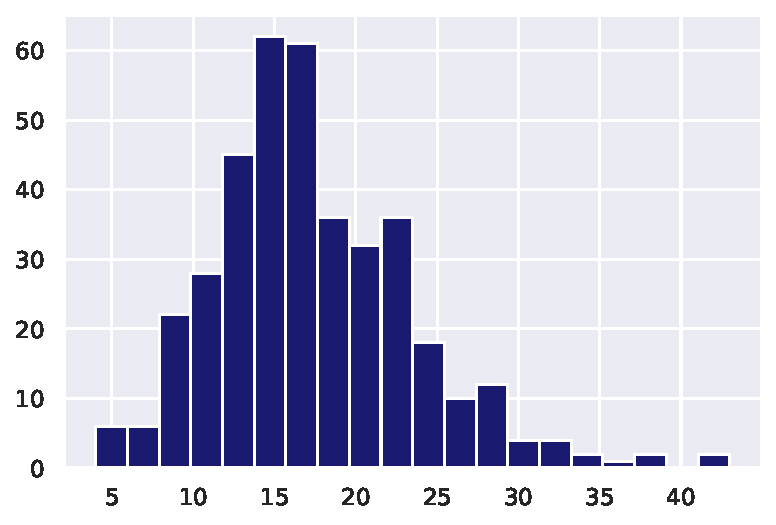
\includegraphics[width=8cm]{degree_distribution_fauxdata.pdf}
    \fonte{The figure was generated with data from \textcite{rds_package}.}
\end{figure}

\begin{figure}[htb]
    \centering
    \caption{\label{fig:rds_faux_data}RDS structure in 
      Faux dataset.}
    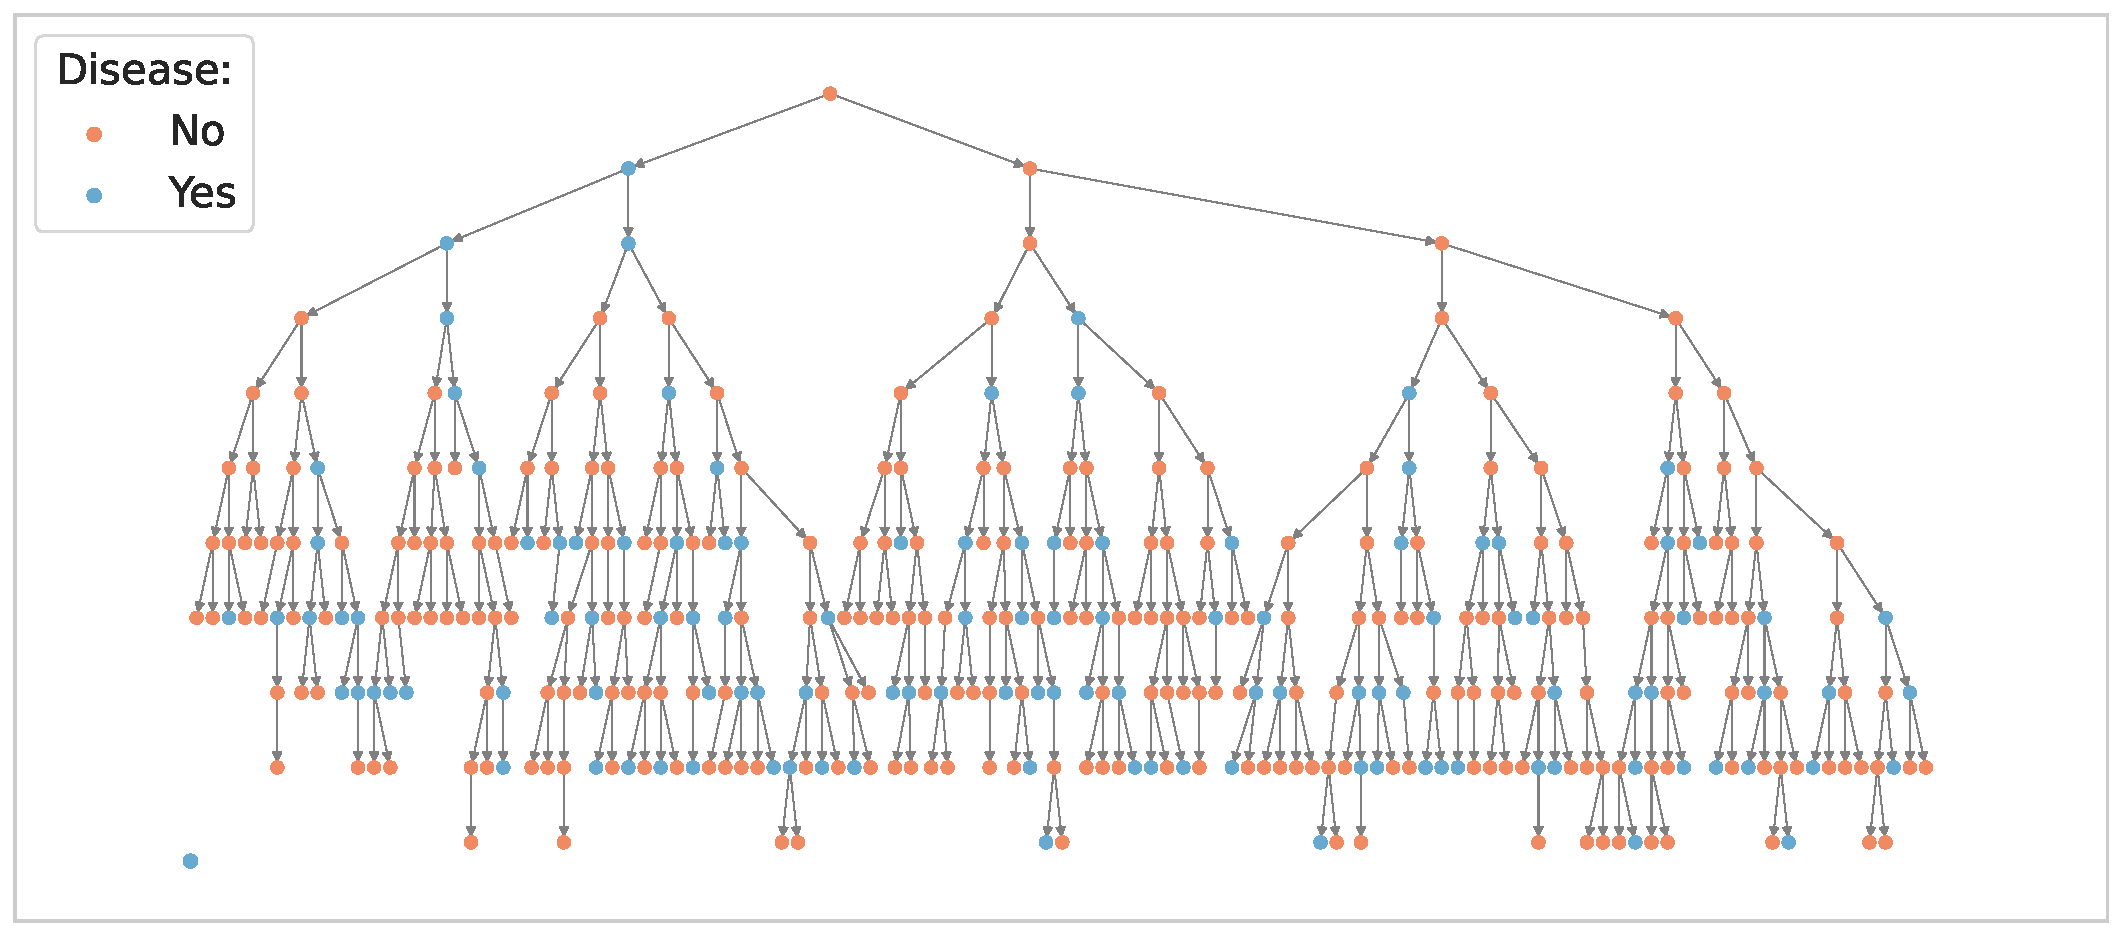
\includegraphics[width=14cm]{rds_faux_data.pdf}
    \fonte{The figure was generated with data from \textcite{rds_package} in
    NetworkX package. The colors indicate the result of the test, yes being positive and no being negative.}
  \end{figure}

We interpret the variable $X$ as the presence of the disease, in
which blue indicates positive and red negative. We define variable $\hat{X}$
to be the diagnostic test result. We omit $X$ and change it by the result of a
diagnostic test with sensitivity $\gamma_s = 0.9$ and specificity $\gamma_e =
0.85$. The prevalence is set to be $0.28$, a little
lower value than the detected in the dataset. The variables $Y$ and $Z$ are
regressors. \autoref{tab:results-estimators-faux-data} presents the biased
results when misclassification is not regarded. The 95\% bootstrap confidence interval
calculated for RDS (SS) estimator was of $(0.352, 0.44)$. 

\begin{table}[htb]
    \centering
    \caption{\label{tab:results-estimators-faux-data}Prevalence point estimation of
    disease $X$ by different approaches in faux dataset}
    \begin{tabular}{ccc}
    \hline
    Estimator & Ignoring misclassification & Frequentist correction \\ \hline
    Naive & 0.385 & 0.314 \\
    RDS (SH) & 0.4 & 0.333 \\
    RDS (VH) & 0.399 & 0.332 \\
    RDS (SS, N=1000) & 0.396 & 0.331 \\
    RDS (SS, N=10000) & 0.398 & 0.314 \\
    RDS-B & 0.4 & 0.334 \\ \hline
    \end{tabular}
    \fonte{Prepared by the author (2021) and based on the results of
    \cite{rds_package}, except for RDS-B, which was self-made. The second
    columns indicate the point estimate without considering the misclassification
    of the test, while the third corrects it with equation \eqref{eq:rogan-estimate-prevalence}.}
\end{table}

Applying our model, we first verify that a gamma prior for $\tau$ is not
indicated, since it puts to much mass in the assumption of correlation. It
caused divergences in the HMC algorithm. Placing a Gumbel prior has the
advantage of allowing $\tau$ be higher. In this case, the posterior mean was
of order $10^{5}$. The parameter $\rho$ had posterior mean of $0.3$. These
results indicate absence of correlation among recruitments. The prevalece
estimate was of $0.25$, a much closer value to $0.28$ than the others, even
with weakly informative priors for the parameters. All the effects include 0
in the centered 50\% credible interval, which indicates that none of them
had effect on the prevalence.

There are two variations of this dataset: madrona and sycamore. The difference
between them is that the latter has extreme seed dependence, while the latter
not. The seed dependence is caused by sampling all the initial individuals
within the infected population. \autoref{fig:bottleneck_plot_madrona} and
\autoref{fig:bottleneck_plot_sycamore} presents the bottleneck plots for each
dataset. This plotting diagnostic introduced by \textcite{gile2015diagnostics}
measures the RDS (VH) estimator for each chain generated by a different seed.
Notice that in sycamore data, all seeds start in the highest part of the graphic
and converge more slowly to the final estimate. 

\begin{figure}
    \centering
    \caption{\label{fig:bottleneck_plot_madrona}Bottleneck plot for faux
    madrona dataset.}
    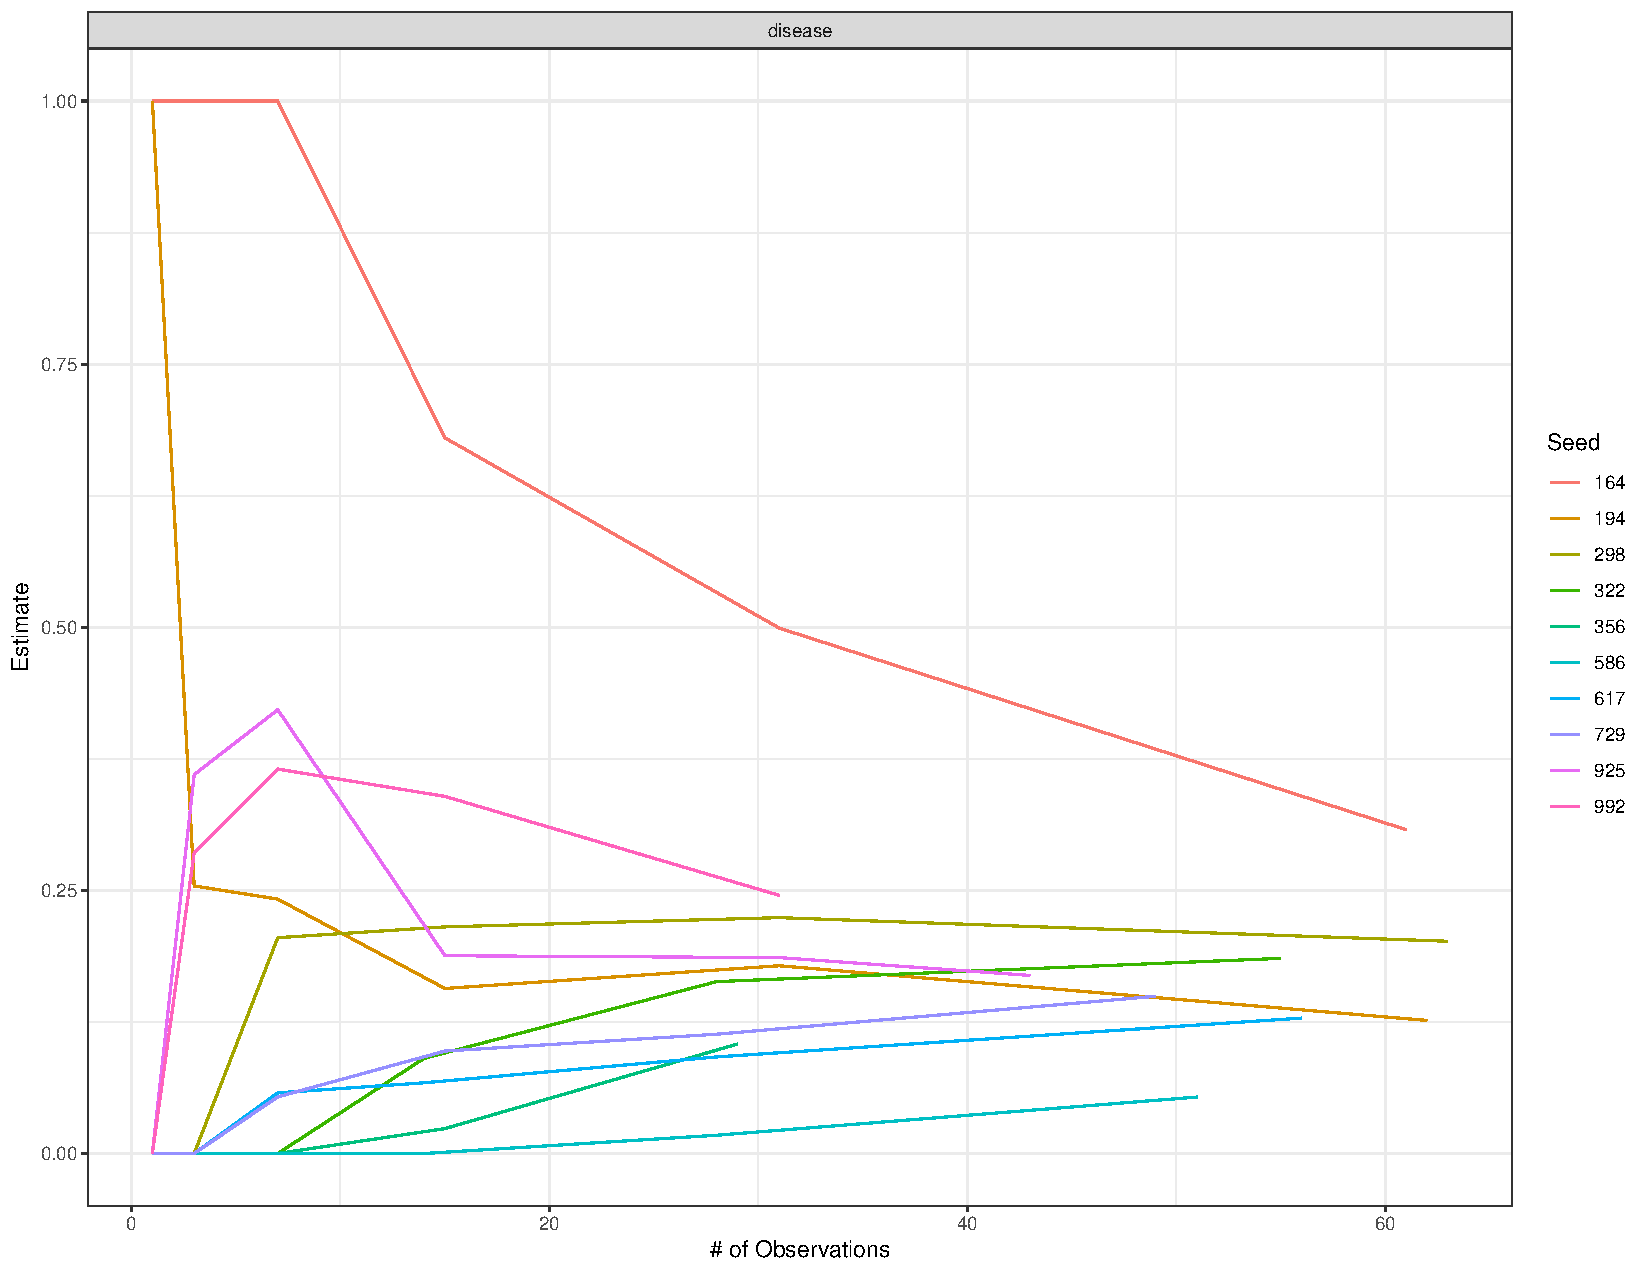
\includegraphics[width=10cm]{faux_madrona_bottleneck_plot.pdf}
    \fonte{Output of \textcite{rds_package}'s package.}
\end{figure}

\begin{figure}
    \centering
    \caption{\label{fig:bottleneck_plot_sycamore}Bottleneck plot for faux
    sycamore dataset.}
    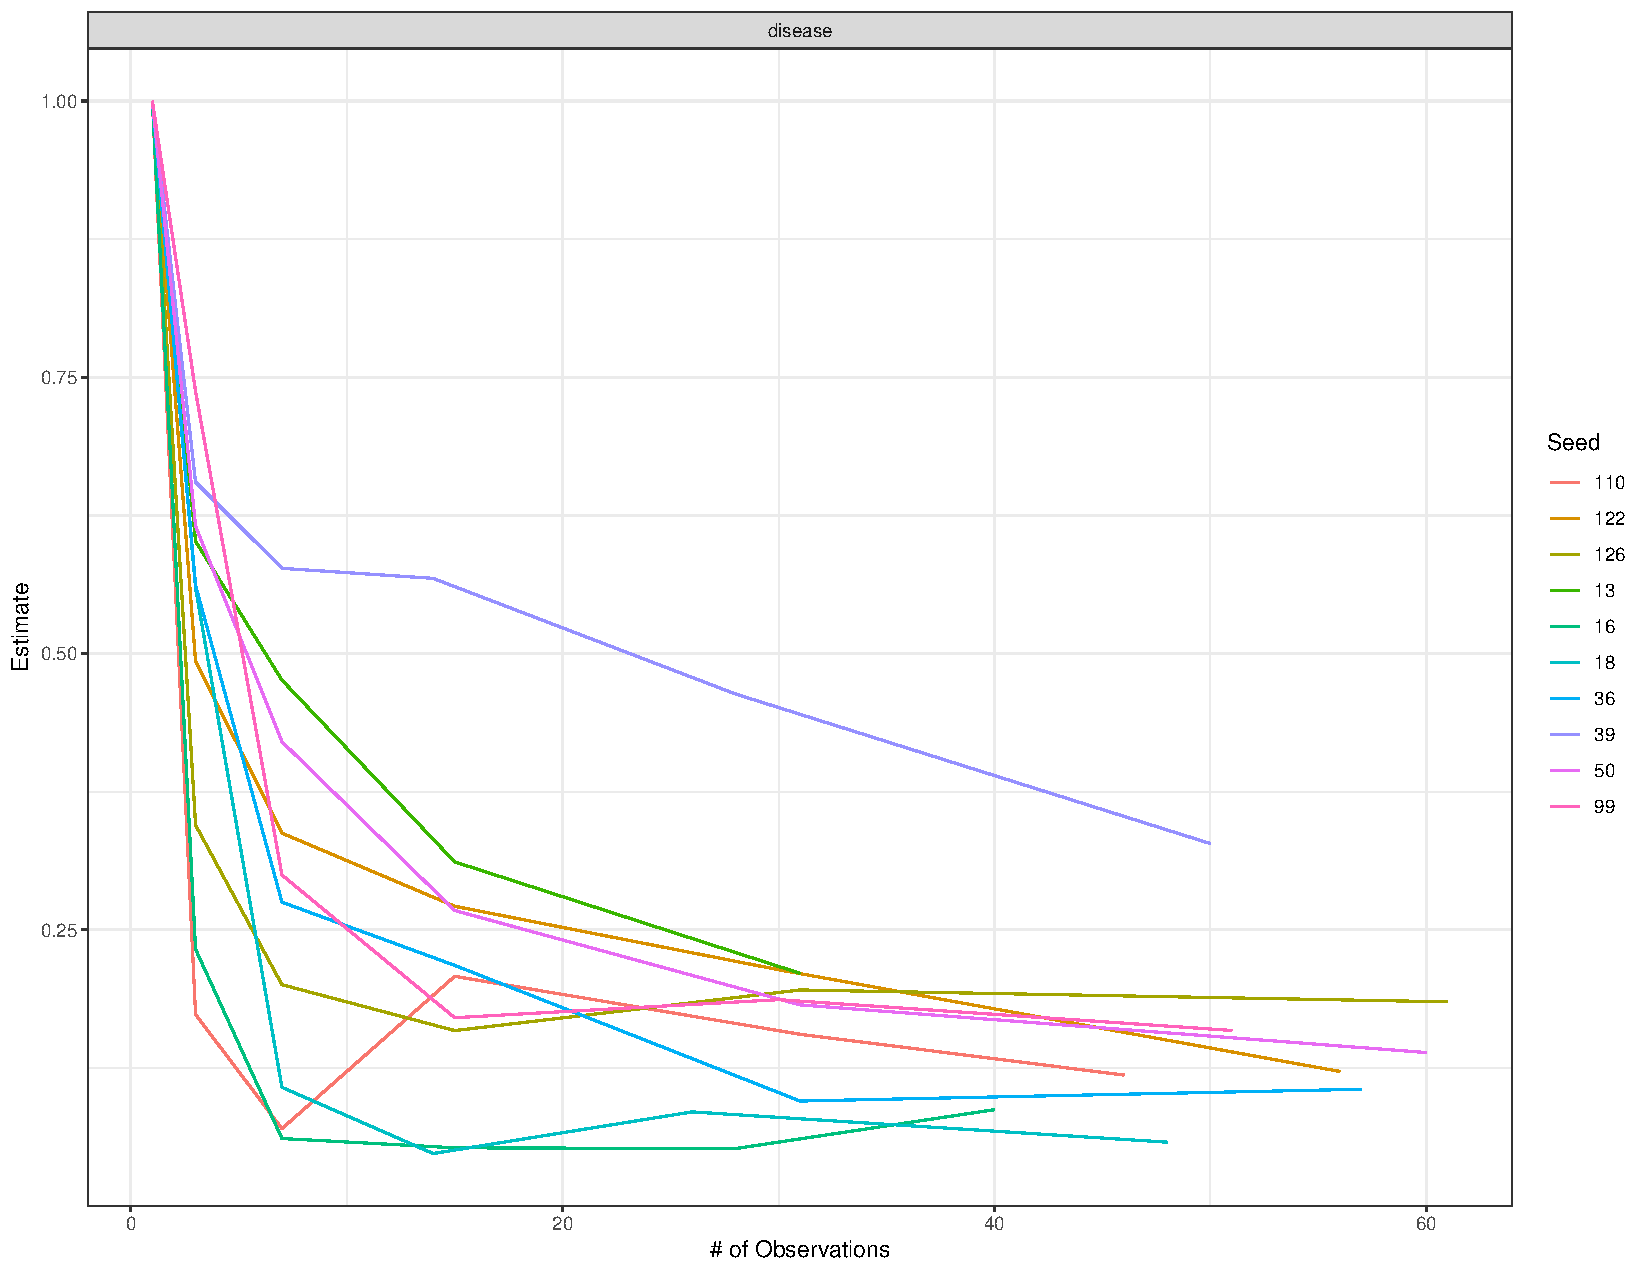
\includegraphics[width=10cm]{faux_sydramore_bottleneck_plot.pdf}
    \fonte{Output of \textcite{rds_package}'s package.}
\end{figure}

Both datasets are built with true prevalence of 0.2 and no covariate are
available. They both have 500 samples. We make the
inferences considering a diagnostic test with sensitivity $\gamma_s = 0.9$ 
and specificity $\gamma_e = 0.85$.
\autoref{tab:results-estimators-faux-madrona-data} shows the resulting
inferences. It seams that the naive estimator got closer to the correct value.
This ocurred because the problems with the naive estimator compensate each
other. All estimators had a bad performance in estimating the prevalence
because the known sensitivity of the test is different from the calculated
within the dataset, i.e., from the individuals without the disease, 90\%
tested negative, which is a greater value than the tru value 85\%. This little difference in
\textcite{rogan1978estimating}'s bias adjustment leads to a high difference in
the estimates, which shows a non-robustness of the estimator. Without considering the
correction for misclassification, the estimated bootstrap 95\% confidence interval was
of $(0.226, 0.279)$ for RDS (SS). 

\begin{table}[htbp]
    \centering
    \caption{\label{tab:results-estimators-faux-madrona-data}Prevalence point estimation of
    disease by different approaches in faux madrona dataset}
    \begin{tabular}{ccc}
    \hline
    Estimator & Ignoring misclassification & Frequentist correction \\ \hline
    Naive & 0.298 & 0.197 \\
    RDS (SH) & 0.228 & 0.104 \\
    RDS (VH) & 0.231 & 0.108 \\
    RDS (SS, N=1000) & 0.253 & 0.137 \\
    RDS (SS, N=10000) & 0.233 & 0.111 \\
    RDS-B & 0.23 & 0.111 \\ \hline
    \end{tabular}
    \fonte{Prepared by the author (2021) and based on the results of
    \cite{rds_package}, except for RDS-B, which was self-made. The second
    columns indicate the point estimate without considering the misclassification
    of the test, while the third corrects it with equation \eqref{eq:rogan-estimate-prevalence}.}
\end{table}

We first consider the informed degree as a covariate of the problem. Proposing
weakly informative priors for $\theta$ and $\beta$, we observe a problem with
$\hat{R}$, which indicates mixing problems among the chains. Increasing the
number of warmup iterations did not solve the problem.
\autoref{fig:rds_model_faux_sycamore_traceplot} shows an identifiability
problem with this covariate in the model. In particular, the posterior
distribution of $\beta$ seems symmetric around 0, which is not a good
inference. Disregarding the degree as covariate, the posterior mean for $\theta$ was of
0.19 (95\% HDI of $0.07-0.31$), which is a pretty good estimate for the
prevalence of 0.2.

\begin{figure}
    \centering
    \caption{\label{fig:rds_model_faux_sycamore_traceplot}Posterior
    distribution and trace plot for $\theta$ and $\beta$ regarding model
    \eqref{model:imperfect-tests-rds}.}
    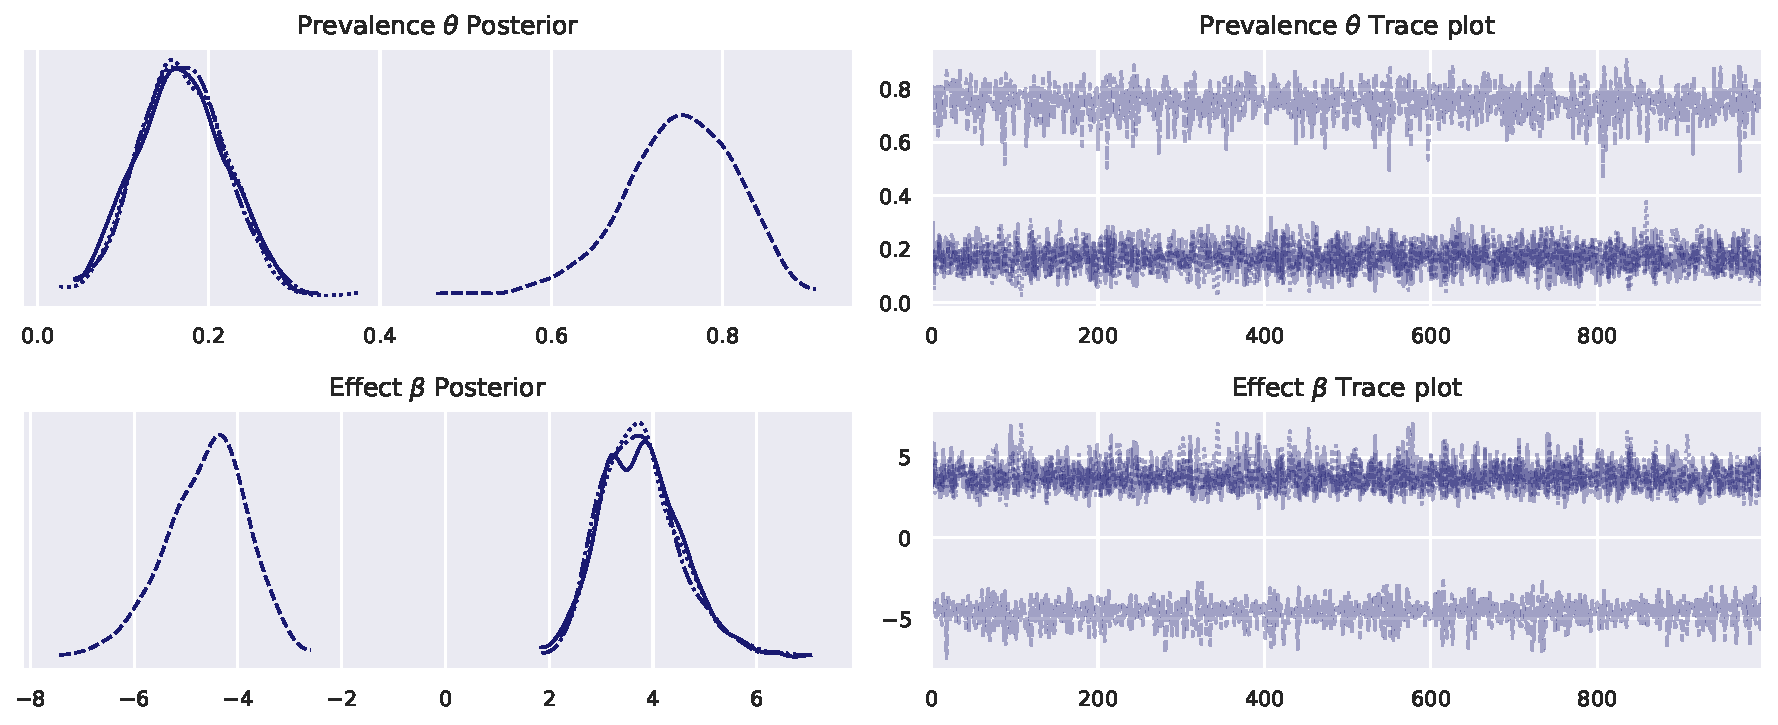
\includegraphics[width=12cm]{rds_model_faux_sycamore_traceplot.pdf}
    \fonte{Prepared by the author (2021) and based on Stan and ArviZ results.}
\end{figure}

For the faux sycamore dataset, the effect of the bias adjustment was less problematic
because the true values for sensitivity and specificity were very close to the
observed in the dataset. In special, RDS (SS) estimator with known population size is
is the most close estimator. Since the seeds influence too much the
inferences, the naive estimator was very far from the true value. 

\begin{table}[htbp]
    \centering
    \caption{\label{tab:results-estimators-faux-sycamore-data}Prevalence point estimation of
    disease by different approaches in faux sycamore dataset}
    \begin{tabular}{ccc}
        \hline
        Estimator & Ignoring misclassification & Frequentist correction \\ \hline
        Naive & 0.354 & 0.272 \\
        RDS (SH) & 0.246 & 0.129 \\
        RDS (VH) & 0.27 & 0.161 \\
        RDS (SS, N=1000) & 0.297 & 0.197 \\
        RDS (SS, N=10000) & 0.273 & 0.164 \\
        RDS-B & 0.273 & 0.164 \\ \hline
        \end{tabular}
    \fonte{Prepared by the author (2021) and based on the results of
    \cite{rds_package}, except for RDS-B, which was self-made. The second
    columns indicate the point estimate without considering the misclassification
    of the test, while the third corrects it with equation \eqref{eq:rogan-estimate-prevalence}.}
\end{table}

Our model had posterior mean of $0.25$ for $\theta$ with 95\% HDI of $0.06 -
0.41$. Since there is more seed dependence and the model does not accommodate
sampling weights, the estimate gets higher than the true value and the
credible interval gets wider.

\section{Project 90 dataset}

Colorado Springs Project 90 was the first prospective assessment of the impact
caused by the network structure in the propagation of infectious diseases. The
Centers for Disease Control and Prevention (CDC) funded this project in 1987
to investigate the dynamics of the human immunodeficiency virus (HIV) in
high-risk heterosexual populations. From 1988 to 1992, the scientists
enumerated 5492 individuals and their connections within the sample. The
populations of the study included female sex workers, men who have sex with
female sex workers, people who injected illicit drugs, and people who have sex
with some injecting drug user \cite[p. 1332]{woodhouse1994mapping}. To form a network of contacts between the
participants, the researchers asked them to describe the relationships with
every other named contact. Only partial information is available for privacy
concerns. 

There are 17 nodes without connections and 108 connected
components in the dataset. The greater has 4430 nodes, while the second has 50
nodes. Therefore, we focus on this bigger connected subgraph. \autoref{fig:graph_project90_degree_distribution} presents the
graph structure and the degree distribution of the nodes. The degree
distribution graph follows the instructions of \textcite[Advanced Topic
3.A]{barabasi2013network} with a log-log plot and logarithmic binning. The
slow decay of the distribution indicates a scale-free network \cite{barabasi2013network}.

\begin{figure}
    \centering
    \caption{\label{fig:graph_project90_degree_distribution}Graph structure and
    degree distribution of the individuals from Project 90 study.}
    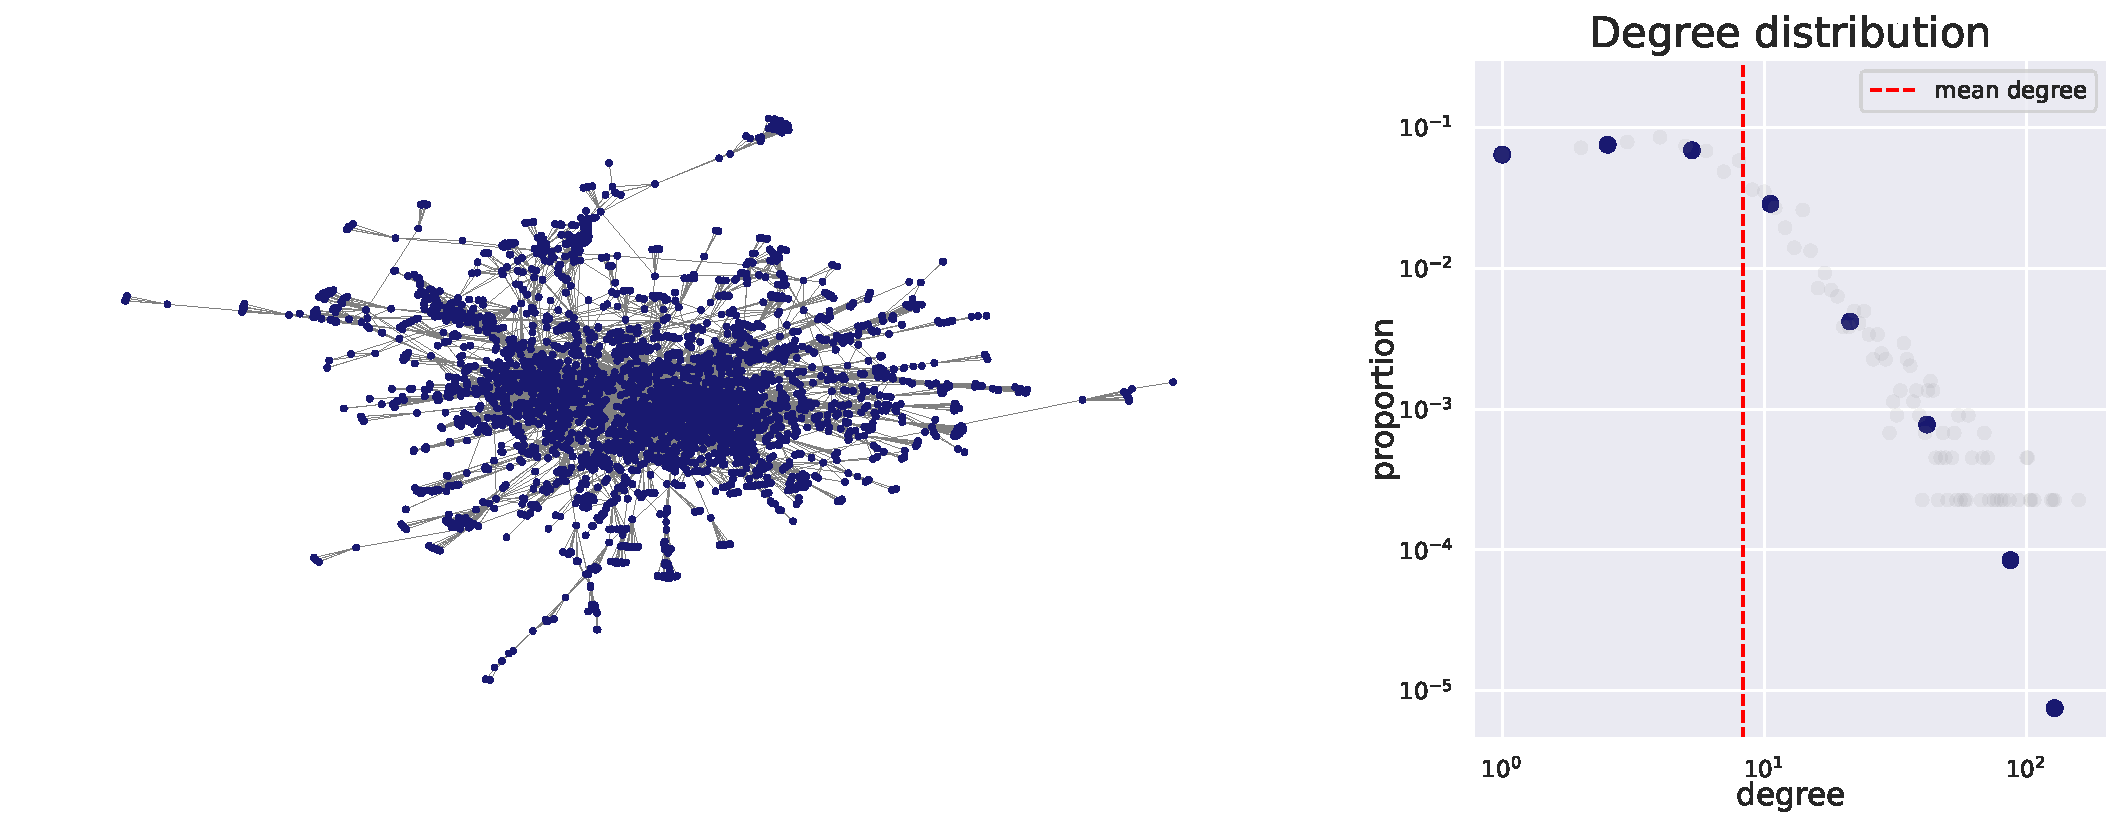
\includegraphics[width=14cm]{graph_projet90_degree_distribution.pdf}
    \fonte{Data from \textcite{project90} and graphics prepared by the author
    (2021). The degree distribution is inn the log-log scale. The grey dots
    represent the degree histogram, while the blue dots calculate the mean for
    each interval defined by logarithmic binning. The construction follows \textcite{barabasi2013network}.}
\end{figure}

\autoref{tab:covariates_project90} summarizes the binary variables of the
dataset. In addition to these variables, the data inform the race of each
individual with 75\% White, 21\%  Black, 1\% Asian/Pacific Islander, 1\%
Native americans, and 0.1\% being others. 93\% of the participants possess the
complete data. We remove the rest from the dataset for simplicity, 
but in a real applications, the uncertainty about this data should be
considered.

\begin{table}[htbp]
    \centering
    \caption{\label{tab:covariates_project90}Proportion distribution for each
    binary variable in Project 90 dataset.}
    \begin{tabular}{cccccccc}
    \hline
    \multirow{2}{*}{Covariate} & \multicolumn{3}{l}{Percentage (\%)} & \multirow{2}{*}{Covariate} & \multicolumn{3}{l}{Percentage (\%)} \\ \cline{2-4} \cline{6-8} 
     & No & Yes & NA &  & No & Yes & NA \\ \hline
    Female & 56.8 & 43.2 & 0.0 & Thief & 91.8 & 2.2 & 6.0 \\
    Sex worker & 88.7 & 5.2 & 6.1 & Retired & 91.1 & 2.9 & 6.0 \\
    Pimp & 92.5 & 1.5 & 6.0 & Housewife & 88.0 & 6.0 & 5.9 \\
    Sex work client & 91.0 & 8.9 & 0.1 & Disabled & 89.9 & 4.1 & 6.0 \\
    Drug dealer & 87.6 & 6.4 & 6.0 & Unemployed & 77.8 & 16.2 & 6.0 \\
    Drug cook & 93.2 & 0.8 & 6.0 & Homeless & 92.8 & 1.2 & 6.0 \\ \hline
    \end{tabular}
    \fonte{Data from \textcite{project90}.}
\end{table}

Since no information about HIV test is available, we use the
column disabled as the outcome of interest. We define the sensitivity
$\gamma_s = 0.9$ and specificity $\gamma_e = 0.85$ for the diagnostic test and
perform a random testing. Moreover, we perform
RDS in this graph following \textcite{baraff2016estimating}, as in Section
\ref{sec:simulated-data-rds-imperfect-tests} and \textcite{crawford2016}, as
in Subsection \ref{sec:including_uncertainty_recruitment_graph}. We compare
the results from our model to the value in the whole network of 0.047. 

Placing priors $\theta \sim \operatorname{Unif}(0,1)$ and $\beta_i \sim
\N(0,1)$, we get a posterior mean for $\theta$ of 0.084 (94\% HDI of $0 -
0.238$) for \textcite{baraff2016estimating}'s simulation and 
0.059 (94\% HDI of $0 - 0.169$) for \textcite{crawford2016}'s model.
All of the effect parameters $\beta$ had 80\% HDI credible intervals
including the value $0$, which indicates no evidence of relation between the variables and
the disabled condition. The prior for $\tau$ was Gumbel with parameter
$\lambda_{\tau} = \log(10)$, while $\rho \sim \operatorname{Unif}(0,1)$. The
posterior mean of $\tau$ was more than 20000 and the posterior mean of $\rho$
was 0.476. In light of the dataset's size and the analysis made in Section
\ref{sec:car-models} about $\rho$, we conclude that there is not much graphical correlation
between recruiters and recruited regarding the disabled condition. Including
gamma prior for $\tau$ did not change the parameter estimates, except for
$\tau$, as expected.

Choosing the seeds within the disabled subpopulation modified the estimate to
0.134 (94\% HDI of $0.0 - 0.333$). The seed dependence bias the results, but
the credible interval is larger, which is a good sign. 